\documentclass[8pt]{article} % use larger type; default would be 10pt

%\usepackage[utf8]{inputenc} % set input encoding (not needed with XeLaTeX)
\usepackage[10pt]{type1ec}          % use only 10pt fonts
\usepackage[T1]{fontenc}
%\usepackage{CJK}
\usepackage{graphicx}
\usepackage{float}
\usepackage{CJKutf8}
\usepackage{subfig}
\usepackage{amsmath}
\usepackage{amsfonts}
\usepackage{hyperref}
\usepackage{enumerate}
\usepackage{enumitem}

\newcommand{\norm}[1]{\left|\left|#1\right|\right|}

\title{Functional Analysis\\Homework I.2}
\author{歐立思\\9822058\\Department of Applied Mathematics\\National Chiao Tung University}
\begin{document}
\begin{CJK}{UTF8}{bsmi}
\maketitle
\end{CJK}
\begin{enumerate}[label=\bfseries\arabic*.]
\item{Basic Operator Theory, Exercises I
	\begin{description}
\item[Exercise 29]{We shall prove equivalence by the following scheme:\\
\begin{description}
\item[$\mathbf{1.}\implies\mathbf{2.}$]{
	$\xi=(\xi_1,\xi_2,\dots)\in span\{x_1,x_2,\dots\}^{\perp}\implies\\
	\forall n\in\mathbb{N},\; <\xi,x_n>=0\implies
	\forall n\in\mathbb{N},\; \xi_n-5\xi_{n+1}+6\xi_{n+2}=0 $
}
\item[$\mathbf{2.}\implies\mathbf{3.}$]{First, let's set up and solve the following system of equations
\[\begin{cases}\frac{\alpha}{2}+\frac{\beta}{3}=\xi_1\\\frac{\alpha}{4}+\frac{\beta}{9}=\xi_2\end{cases}\]
It is obvious that system is non-degenerated, and therefore solvable for any values of right-hand side. Now, let's show by induction that
$\xi_n=\frac{\alpha}{2^n}+\frac{\beta}{3^n}$. Shall we succeed, we may conclude that $\xi=
\frac{\alpha}{2}(1,\frac{1}{2},\frac{1}{4},\frac{1}{8},\dots)+\frac{\beta}{3}
(1,\frac{1}{3},\frac{1}{9},\frac{1}{27},\dots)$. Now, from the choice of $\alpha$ and $\beta$ we already have our base case ($n=1,2$). Therefore,
all we may proceed as follows
\[6\xi_{n+2}=5\xi_{n+1}-\xi_n=5\frac{\alpha}{2^{n+1}}+5\frac{\beta}{3^{n+1}}-\frac{\alpha}{2^n}-\frac{\beta}{3^n}=\frac{6\alpha}{2^{n+2}}+\frac{
	6\beta}{3^{n+2}}\]
}
\item[$\mathbf{3.}\implies\mathbf{1.}$]{It is sufficient to show that both $(1,\frac{1}{2},\frac{1}{4},\frac{1}{8},\dots)$ and 
$(1,\frac{1}{3},\frac{1}{9},\frac{1}{27},\dots)$ are normal to all of $x_n$. Both things are easy to see if one will notice obvious relations,
that hold for $\forall n \in \mathbb{Z}$
\[\frac{6}{2^{n+2}}-\frac{5}{2^{n+1}}+\frac{1}{2^n}=0\]\[\frac{6}{3^{n+3}}-\frac{5}{3^{n+1}}+\frac{1}{3^n}=0\]
}
\end{description}}
\item[Exercise 32]{Using the reasoning similar to the previous exercise one may show, that $y\in sp\{x_1,x_2,\dots\}^\perp \iff y=\alpha(1,\frac{-1}{2},
\frac{1}{4},\dots)$}
Now, since the closure of a subspace is the same as orthogonal complement taken two times, it is sufficient to show that \textit{none} of
$y_i$ is normal to $(1,\frac{-1}{2},\frac{1}{4},\dots)$. But this is obvious from definitions.
\item[Exercise 43]{Before we start, let us make a brief observation. 
\begin{figure}[H]
\centering
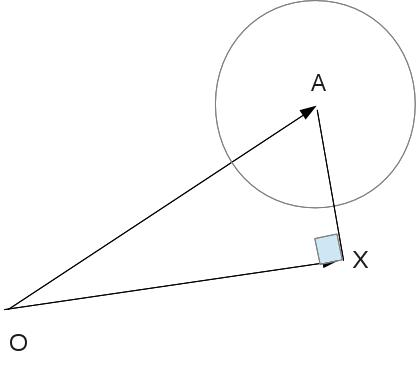
\includegraphics[width=0.6\textwidth]{funcAn_hw2_pic1}
\end{figure}
Picture above suggests some basic geometric reasoning. On it, we depict the cross-section of the $l_2$ by the plane going through the vectors
$x$ and $\alpha_0$. The sphere $\norm{z-\alpha_0}\leq R_0$ is drawn as circle, $OX$ represents line $\lambda x$, $\vec{OA}=\alpha_0$ and angle
$\angle OXA$ is assumed to be right (i.e. equal to $\pi/2$). From this one immediately sees that all we need is to compare $R_0$ and $\norm{\vec{
	AX}}$. In turn, $\norm{\vec{AX}}=\norm{\alpha_0}\sin \alpha$, where $\cos \alpha=\frac{<\alpha_0,\vec{OX}>}{\norm{\alpha_0}
	\norm{\vec{OX}}}$
	\begin{enumerate}[label=(\alph*)]
\item{\[\cos \alpha=\frac{1/\sqrt{3}}{\sqrt{3}/\sqrt{2}}=\frac{\sqrt{2}}{3}\implies \sin \alpha=\frac{\sqrt{7}}{3}\]
	\[\norm{\vec{AX}}=\frac{\sqrt{7}}{3}>R_0=1/2\]
	Therefore, \textit{line does not intersect the ball}
}
\item{\[cos \alpha=0 \implies \sin \alpha=1\]
\[\norm{\vec{AX}}=\frac{2}{\sqrt{3}}<R_0=\frac{4}{3}\]
Therefore, \textit{line intersects the ball}
	}
\end{enumerate}}
\item[Exercise 50(a)]{\begin{enumerate}[label=(\alph*)]
	\item{Assume, seeking the contradiction, that for each $m \in \mathbb{N}$ we have linearly dependent system of vectors
	$\{y^{(m)}_i\}_{i=1}^n$ such that $\norm{z_i-y^{(m)}_i}<
	1/m$. Let use consider the $G_m$ - the Gram determinant of $\{y^{(m)}_i\}_{i=1}^n$. Since for each $m$ the system is linearly dependent,
	Gram determinant is always zero. On the other hand, since for each $i=1,2,\dots,n$ we have $y^{(m)}_i \to z_i$ as $m\to\infty$, then 
	$<y^{(m)}_i,z_j>\to<z_i,z_j>$ and therefore $G_m\to G$, where G denotes Gram determinant of $\{z_i\}_{i=1}^n$ and is nonzero. Therefore,
	sequence consisting of zeros has nonzero limit. Contradiction.
	}
	\end{enumerate}
}
\item[Exercise 51]{Recall first that given linearly independent system of vectors $A=\{a_1,a_2,\dots,a_n\}$ we may express the result of Gram-
Schmidt process by the non-recursive formula involving "formal determinants", that is
\[\alpha_i=\frac{1}{\sqrt{G_{j-1}G_j}}
\begin{vmatrix}
\langle a_1, a_1 \rangle & \langle a_2, a_1 \rangle & \dots & \langle a_j, a_1 \rangle \\
\langle a_1, a_2 \rangle & \langle a_2, a_2 \rangle & \dots & \langle a_j, a_2 \rangle \\
\vdots & \vdots & \ddots & \vdots \\
\langle a_1, a_{j-1} \rangle & \langle a_2, a_{j-1} \rangle & \dots &
\langle a_j, a_{j-1} \rangle \\
a_1 & a_2 & \dots & a_j \end{vmatrix} \;\text{, for }i=1,2,\dots n\]
where $G_i$ is a Gram determinant of $\{a_1,a_2,\dots,a_j\}$ and vectors $\{\alpha_i\}_{i=1}^n$ are orthonormal and generate
the same span as $a_i$. 
From the formula above one sees directly that $\alpha_i$ depend continuously on $a_i$. Therefore, we will define $\alpha_i$ and $\beta_i$ to be
orthonormal families obtained by applying Gram-Schmidt process to the $a_i$ and $b_i$ respectively (from the beginning we assume that $\delta>0$
is small enough so that $b_i$ are linearly independent - see previous problem). And because $\alpha_i$ (respectively, $\beta_i$) depend
continuously on $a_i$ (respectively, $b_i$) we may assume that $\forall i \in \{1,2,\dots,n\},\;\norm{\alpha_i-\beta_i}<\delta$ where $\delta>0$ 
should be chosen in order to satisfy $\norm{y_A-y_B}\leq \epsilon \norm{y}$ for $\epsilon>0$ given. But this is easy. In fact
\[\norm{y_A-y_B}=\norm{\sum_{i=1}^n<y,\alpha_i>\alpha_i-\sum_{i=1}^n<y,\beta_i>\beta_i}\leq\sum_{i=1}^n\norm{<y,\alpha_i>\alpha_i-<y,\beta_i>\beta_i}=\]
\[=\sum_{i=1}^n\norm{<y,\alpha_i>\alpha_i-<y,\beta_i>\alpha_i+<y,\beta_i>\alpha_i-<y,\beta_i>\beta_i}=\]
\[=\sum_{i=1}^n\norm{<y,\alpha_i-\beta_i>\alpha_i+<y,\beta_i>(\alpha_i-\beta_i)}\leq\]
\[\leq\sum_{i=1}^n\norm{y}\norm{\alpha_i-\beta_i}\norm{\alpha_i}
+\norm{y}\norm{\beta_i}\norm{\alpha_i-\beta_i}=\norm{y}\sum_{i=1}^n \norm{\alpha_i-\beta_i}(\norm{\alpha_i}+\norm{\beta_i})<\norm{y}\epsilon\]
The last inequality requires $\sum_{i=1}^n \norm{\alpha_i-\beta_i}(\norm{\alpha_i}+\norm{\beta_i})\leq
\sum_{i=1}^n (\norm{\alpha_i}+\norm{\beta_i})^2$ to be small, but this holds as soon as
$\norm{\alpha_i-\beta_i}$ is small enough for all $i$. To be more precise, we need $\delta<\sqrt{\frac{\epsilon}{n}}$
	}
\item[Exercise 69]{\begin{enumerate}[label=(\alph*)]
\item{Applying the logic similar to used in problem 29, we see that $L_1=\text{sp}\{(1,\frac{-1}{2},\frac{1}{4},\frac{-1}{8},\dots)\}^\perp$
and $L_2=\text{sp}\{(1,\frac{-1}{3},\frac{1}{9},\frac{-1}{27},\dots)\}^\perp$
Therefore, $L_1\cap L_2=\text{sp}\{(1,\frac{-1}{2},\frac{1}{4},\frac{-1}{8},\dots),(1,\frac{-1}{3},\frac{1}{9},\frac{-1}{27},\dots)\}^\perp$.
Again, following the logic used in problem 29 we may show by induction that 
$(\eta_1,\eta_2,\dots)\in\text{sp}\{(1,\frac{-1}{2},\frac{1}{4},\frac{-1}{8},\dots),(1,\frac{-1}{3},\frac{1}{9},\frac{-1}{27},\dots)\}$ 
if $\forall k\in\mathbb{N},\;6\eta_{k+2}+5\eta_{k+1}+\eta_k=0$. To show the opposite direction ("only if"), and therefore finish this item, we do
straightforward some calculations
\[(\eta_1,\eta_2,\dots)\in\text{sp}\{(1,\frac{-1}{2},\frac{1}{4},\frac{-1}{8},\dots),(1,\frac{-1}{3},\frac{1}{9},\frac{-1}{27},\dots)\}\implies\]
\[\implies \eta_i=\frac{\alpha}{(-2)^{i-1}}+\frac{\beta}{(-3)^{i-1}}\implies\]
\[\implies \forall k\in\mathbb{N},\;6\eta_{k+2}+5\eta_{k+1}+\eta_k=\alpha\frac{6-10+4}{(-2)^{k+1}}+\beta\frac{6-15+9}{(-3)^{k+1}}=0\]
}
\item{Notice that $\eta=(\eta_1,\eta_2,\dots)\in\text{sp}\{(1,5,6,\dots),(0,1,5,6,\dots),\dots\}^\perp\iff \forall k\in\mathbb{N},
\;6\eta_{k+2}+5\eta_{k+1}+\eta_k=0$. Therefore, in the light of previous item,
$x\in L_1\cap L_2 \iff \forall \eta\in \text{sp}\{(1,5,6,\dots),(0,1,5,6,\dots),\dots\}^\perp,\;<x,\eta>=0 \iff
x\in\text{sp}\{(1,5,6,\dots),(0,1,5,6,\dots),\dots\}^{\perp\perp}=\overline{\text{sp}}\{(1,5,6,\dots),(0,1,5,6,\dots),\dots\}$. Therefore,
$L_1\cap L_2=\overline{\text{sp}}\{(1,5,6,\dots),(0,1,5,6,\dots),\dots\}$
}
\end{enumerate}
}
\end{description}
	}
\item{Recall that Legendre polynomials $P_n(x)$ investigated in the class have the following properties:\begin{itemize}
\item{$\int_{-1}^1 P_n(t)t^kdt=0,\,k=0,1,\dots,n-1;$}
\item{$P_n(1)=1,\,n\leq0$}
\end{itemize}
Thus, one immediately sees that polynomials $f_n(k)$ defined as $f_n(x):=P_n(2\frac{x-a}{b-a}-1)$ has the properties required in the problem.
Indeed, $f_n(b)=P_n(1)=1$ and the statement $\int_a^b f_n(t)t^kdt=0,\,k=0,1,\dots,n-1;$ can be shown as follows.\[
\int_a^b f_n(x)x^k dx=\int_a^b P_n(2\frac{x-a}{b-a}-1) x^k dx=\frac{b-a}{2}\int_{-1}^1 P_n(t)(\frac{b-a}{2}(t+1)+a)^kdx=\]
\[=\frac{b-a}{2}\int_{-1}^1P_n(t)\sum_{i=0}^k(\frac{b-a}{2})^it^i (\frac{b+a}{2})^{(k-i)}dt=\]
\[=\sum_{i=0}^k(\frac{b-a}{2})^{(i+1)}
(\frac{b+a}{2})^{(k-i)}\int_{-1}^1 P_n(t)t^i dt=\sum_{i=0}^k(\frac{b-a}{2})^{(i+1)}(\frac{b+a}{2})^{(k-i)}\cdot0=0\]
Finally, to show that the zeros of $f_n(x)$ are distinct real numbers in $(a,b)$ we will do as follows. First, assume that $f_n(x)$ has some some
double or complex roots. Then, $f_n(x)=(x-x_1)(x-x_2)\dots(x-x_k)p_1(x)p_2(x)\dots p_l(x)$, where $p_i(x)$ are of the form $p_i(x)=(x-\alpha_i)^2$
or $p_i(x)=(x-\alpha_i)(x-\bar{\alpha}_i)$ and are formed from the presence of multiple roots or complex roots (latter will occur in
conjugate pairs). Since polynomials $p_i(x)$ are non-negative (on real line),
 we may consider the polynomial $t(x)=(x-x_1)\dots(x-x_k)$ of degree smaller than $n$.
Then, we should have $\int_a^b f_n(x)t(x)dx=0$. But $\int_a^b f_n(x)t(x)dx=\int_a^b (x-x_1)^2\dots(x-x_k)^2\dots p_1(x)\dots p_l(x)dx>0$ and we
arrived at contradiction. Finally, assume that some zero $x_0$ of $f_n(x)$ is outside $(a,b)$. Then, $f_n(x)=(x-x_0)q(x)$ and since degree
of $q(x)$ is smaller than $n$ we must have $\int_a^b f_n(x)q(x)dx=\int_a^b (x-x_0)q^2(x)dx=0$. But $q^2(x)$ is non-negative and $x-x_0$ \textit{
	does not change sign} on $(a,b)$, therefore expression in the last integral does not change sign on $(a,b)$ and cannot give zero
	integral, unless it's equal to zero, which is not true. We again arrived at contradiction.
}
\item{
	\begin{enumerate}[label=(\arabic*)]
	\item{First, it is clear that so defined $q_j(x)$ are in fact Lagrange interpolation polynomials and $q_j(x_i)=\delta_{ij}$, where 
	$\delta_{ij}$ is Kronekecker delta (equal to one if $i=j$ and zero otherwise). Now, for $\text{deg}(P(x))\leq 2n-1$ we have
	\[P(x)=q(x)f_n(x)+r(x),\;\text{deg}(q(x)) \leq n-1,\;\text{deg}(r(x)) \leq n-1\]
	\[r(x_i)=P(x_i)-q(x_i)f_n(x_i)=P(x_i)-q(x_i)\cdot 0=P(x_i)\]
	Also, since $\text{deg}(r(x)) \leq n-1$ we may apply Lagrange polynomials and write $r(x)=\sum_{i=1}^n r(x_i)q_i(x)=\sum_{i=1}^n P(x_i)
	q_i(x)\implies \sum_{i=1}^n a_i P(x_i)=\int_a^b r(x)dx=\int_a^b P(x)dx-\int_a^b q(x)f_n(x)dx=\int_a^bP(x)dx$. Clearly,
	$\int_a^b q(x)f_n(x)dx=0$ because of degree of $q(x)$ and properties of $f_n(x)$.}
	\item{Fix $j$ and consider $P(x)=(x-x_1)^2(x-x_2)^2\dots(x-x_{j-1})^2(x-x_{j+1})^2\dots(x-x_n)^2\geq 0$. According to what was proved above
	\[\sum_{i=1}^n a_iP(x_i)=\int_a^b P(x)>0\]Now, $i\neq j\implies P(x_i)=0,\;P(x_j)>0$. Therefore, \[0<\sum_{i=1}^n a_iP(x_i)=a_jP(x_j)
	\implies 0<a_j\]
	}
	\end{enumerate}
}
\item{Fix $i=1,\dots,n$ and let's consider the polynomial $P(x)=f_n(x)(x-t_1)\dots(x-t_{i-1})(x-t_{i+1})\dots(x-t_n)$. Let's make a few
observations
\begin{itemize}
\item{$\int_a^b P(x)=0$ by the properties of $f_n(x)$ and because $\text{deg}((x-t_1)\dots(x-t_{i-1})(x-t_{i+1})\dots(x-t_n))=n-1<n$}
\item{$j\neq i\implies P(t_j)=0$}
\end{itemize}
Therefore, \[0=\int_a^b P(x)=a_i P(t_i)\implies P(t_i)=0\] Hence, since $j\neq i\implies t_j\neq t_i$ we have $f_n(t_i)=0$ and $t_i$ is zero of
$f_n$. Since $t_i$ above was chosen arbitrarily, argument applies to all of them, therefore all of them are zeros of $f_n(x)$.
}
\end{enumerate}
\end{document}
